\documentclass[11pt]{article}

\usepackage[margin=1in]{geometry}
\usepackage{amsmath, amssymb}
\usepackage{booktabs}
\usepackage{siunitx}
\usepackage{graphicx}
\usepackage{natbib}
\usepackage[hidelinks]{hyperref}
\usepackage{authblk}
\usepackage{orcidlink}

\sisetup{detect-weight=true, detect-family=true}
\graphicspath{{../stock_project/reports/figures_v2/}}
\bibliographystyle{plainnat}

\title{\bfseries A GARCH-Scaled Hierarchical Bayesian Model for Calibrated
Daily Return Densities: Evidence from Large-Cap Technology Stocks, 2016--2025}

\author[1]{R.\,O.\ Attafuah}
\author[2]{B.\,A.\ Adjei}
\author[3]{K.\ Incoom-Koomson}
\affil[1]{Miami University}
\affil[2]{Texas State University}
\affil[3]{Georgia State University}
\date{}

\begin{document}
\maketitle

\begin{abstract}
\noindent
Forecasts of daily equity returns are usually evaluated on point accuracy, yet
most practical uses, such as risk limits, position sizing and option pricing, require a
predictive \emph{distribution}. We develop and evaluate a hierarchical Bayesian
model that supplies one. The specification treats a GARCH(1,1)-$t$ conditional
standard deviation as a known observation scale, pools intercepts across assets,
places a horseshoe prior on the mean coefficients so that predictor selection
occurs inside the posterior, and uses Student-$t$ innovations with a scale
calibrated on validation data. Estimation is by blocked Gibbs sampling with all
conditionals in closed form; the sampler recovers known parameters on synthetic
data and satisfies standard convergence diagnostics.

On a balanced panel of eight large-capitalisation United States technology
stocks over 2016--2025, evaluated on a held-out window spanning the 2022--2023
monetary tightening cycle, the model attains the best logarithmic score and
continuous ranked probability score among all specifications considered,
improving on a ridge-plus-GARCH benchmark by $0.126$ nats
($p<0.00001$), and reduces mean absolute interval-coverage error to $0.022$ from
$0.030$. Partial pooling delivers a further practical benefit: for an asset
excluded from estimation entirely, the model still produces intervals attaining
$87\%$ coverage at the $90\%$ nominal level, with a logarithmic score within
$0.005$ nats of the same model estimated with that asset included.

Decomposing the gain in predictive density over a null forecast shows where the
value originates: the conditional variance contributes $54\%$ and the shape of
the predictive distribution a further $45\%$, while the conditional mean
contributes $0.7\%$. Consistent with the out-of-sample evidence of Welch and
Goyal (2008) and Timmermann (2008), no specification improves on a per-ticker
historical average for the conditional mean, which is precisely why modelling
effort at this horizon is better directed at the second moment and the
distributional shape. We additionally document a silent failure mode:
standardising non-stationary macroeconomic levels on a fixed estimation origin
sends held-out inputs to $8.7$ training standard deviations and produces
out-of-sample $R^2$ as low as $-10\,425\%$ with no error raised. All code, audit
scripts and pinned dependencies are released.
\end{abstract}

\noindent\textbf{Keywords:} density forecasting; forecast calibration;
hierarchical Bayesian models; GARCH; cross-asset transfer

% !TEX root = main.tex

\section{Introduction}
\label{sec:intro}

Between 2016 and 2025, large-capitalisation United States technology equities
traded through several distinct macro-financial regimes: an extended period of
near-zero policy rates, the COVID-19 market dislocation of March 2020, the most
rapid monetary tightening cycle since the early 1980s beginning in 2022, and the
partial normalisation of rates that followed. These episodes produced pronounced
volatility clustering, heavy-tailed daily returns, and repeated shifts in the
joint distribution of returns and macroeconomic state variables, features long
documented as stylised facts of asset returns \citep{cont2001empirical}. Such
conditions are hostile to forecasting models estimated under an assumption of
covariance stationarity, and they reproduce at the level of a portfolio a
persistent finding of the empirical finance literature: predictive relations
that appear stable in sample frequently deteriorate out of sample
\citep{welch2008comprehensive, timmermann2008elusive}. As \citet{west2020bayesian}
argues, structure uncertainty then becomes as consequential as parameter
uncertainty, since the analyst must decide not only what the coefficients are
but which model, if any, remains adequate as the regime changes.

There are sound theoretical grounds for conditioning return forecasts on
macro-financial information. Multifactor asset pricing theory implies that
innovations in systematic state variables are priced in equity returns
\citep{chen1986economic}. Empirically, unanticipated changes in the federal funds
rate induce large and statistically significant equity market responses
\citep{bernanke2005explains}; option-implied volatility, summarised by the CBOE
Volatility Index, is contemporaneously and negatively associated with returns
\citep{whaley2000investor}; and comovement with the broad market index remains
the dominant source of systematic variation in individual stock returns. Recent
data-driven studies confirm that volatility and uncertainty measures rank among
the most influential predictors of index returns \citep{latif2025integrating},
and that volatility transmission across markets is itself time varying
\citep{agrawal2026volatility}. The unresolved methodological question is
therefore not whether such variables carry information, but how they should enter
the forecasting model and how the resulting predictive uncertainty should be
quantified.

This paper approaches that question constructively. Most practical uses of a
return forecast, such as setting a risk limit, sizing a position or pricing
an option, require a predictive \emph{distribution} rather than a point estimate,
yet the forecasting literature is dominated by evaluations of conditional-mean
accuracy. We develop a model that supplies a calibrated distribution, and we
establish which of its components does the work.

The specification is a hierarchical Bayesian regression with four features. It
treats a GARCH(1,1)-$t$ conditional standard deviation as a \emph{known}
observation-level scale, so the model does not have to relearn volatility
clustering and a single scalar measures whether that scale is correctly sized.
It pools intercepts across assets, which allows an asset absent from estimation
to be forecast by integrating its intercept over the population distribution. It
places a horseshoe prior \citep{carvalho2010horseshoe} on the mean coefficients,
so that predictor selection occurs inside the posterior with uncertainty
attached rather than as a screening step beforehand. And it uses Student-$t$
innovations with a scale calibrated on validation data, which separates
tail behaviour from scale. Estimation is by blocked Gibbs sampling with every
conditional in closed form.

The evaluation is a controlled comparison on a balanced panel of eight large-cap
technology stocks over 2016--2025, with the effective federal funds rate, the
ten-year Treasury yield, the VIX and a market proxy as macro-financial
conditioning information. Competing specifications (naive baselines, pooled
ridge, a pooled random forest, three GARCH-family volatility models and four
sequence architectures) are estimated on an identical feature set and scored on
a strictly held-out window spanning the tightening cycle and its aftermath.
Point accuracy is assessed by root mean squared error and out-of-sample $R^2$;
probabilistic adequacy by logarithmic score, continuous ranked probability score
and interval calibration. Every comparison is tested by Diebold--Mariano rather
than ranked.

We report four findings. First, the proposed model attains the best logarithmic
score and CRPS among all specifications considered, improving on a
ridge-plus-GARCH benchmark by $0.126$ nats ($p<0.00001$), and reduces mean
absolute interval-coverage error to $0.022$ from $0.030$. Second, partial pooling
yields calibrated intervals for an asset with no estimation history at all,
attaining $87\%$ coverage at the $90\%$ nominal level and a logarithmic score
within $0.005$ nats of the same model estimated with that asset included. Third,
decomposing the gain in predictive density over a null forecast locates its
source: the conditional variance contributes $54\%$ and the shape of the
predictive distribution a further $45\%$, while the conditional mean contributes
$0.7\%$, detectable at $p=0.029$ and economically negligible. Fourth,
consistent with \citet{welch2008comprehensive} and \citet{timmermann2008elusive},
no specification improves on a per-ticker historical average for the conditional
mean, a result that survives disaggregation to individual assets and correction
for multiple testing, and which is precisely why modelling effort at this horizon
is better directed at the second moment and the distributional shape.

We also document a failure mode that is silent rather than merely severe.
Standardising non-stationary macroeconomic levels on a fixed estimation origin
sends held-out inputs far outside the range seen in estimation, and every model
with an unbounded output head extrapolates along them, producing out-of-sample
$R^2$ as low as $-10\,425\%$ with no exception raised and no implausible training
diagnostic. Because the defect is detectable only by auditing predictor
distributions across splits and the scale of the predictions themselves, both
audits are released with the code.

The remainder of the paper reviews the relevant literature, describes the data
and methodology, reports the empirical results, and concludes with
recommendations for practice.

% !TEX root = main.tex

\section{Literature Review}
\label{sec:literature}

\subsection{Classical time-series models and the limits of return predictability}

The autoregressive integrated moving average framework of \citet{box1970time}
remains the canonical linear model for the conditional mean of a univariate
series and the natural benchmark against which richer specifications are judged.
Its known limitation in financial applications lies in the second moment: daily
returns exhibit conditional heteroskedasticity, which motivated the ARCH model of
\citet{engle1982autoregressive} and its GARCH generalisation
\citep{bollerslev1986generalized}, and which implies that a correctly specified
linear conditional-mean model may still misstate predictive uncertainty by a wide
margin. A second limitation concerns the conditional mean itself. In a
comprehensive out-of-sample audit, \citet{welch2008comprehensive} found that most
proposed return predictors fail to improve upon the historical average, and
\citet{timmermann2008elusive} characterised return predictability as local and
episodic---present in short-lived pockets rather than as a stable population
property. Forecast combination offers partial insurance against this instability
\citep{rapach2010out}, but the collective evidence establishes a demanding
baseline: any gain claimed for a more elaborate model must survive genuine
out-of-sample evaluation over heterogeneous regimes.

\subsection{Machine learning approaches}

Machine learning methods relax the linearity restriction at the cost of a larger
effective parameter space. Random forests \citep{breiman2001random} control
overfitting through bootstrap aggregation of decorrelated trees and provide
internal measures of predictor importance, properties that make them a common
nonlinear benchmark in return forecasting. In the most systematic comparison to
date, \citet{gu2020empirical} showed that regression trees and neural networks
yield economically significant improvements in measuring equity risk premia,
attributing the gains chiefly to nonlinear predictor interactions that linear
methods miss. For sequence models, the LSTM architecture
\citep{hochreiter1997long} was shown by \citet{fischer2018deep} to outperform
random forests and logistic regression in classifying daily S\&P~500 constituent
returns, although the documented profitability of the strategy declined in later
subperiods---an instability consistent with the pocketed predictability described
above. Subsequent applied work has extended these architectures with
macroeconomic inputs and hybrid convolutional--recurrent designs
\citep{latif2025integrating}. Two limitations recur throughout this literature:
the fitted models are difficult to interpret, and their outputs are point
predictions unaccompanied by a distributional statement.

A third limitation is less often discussed and is central to this paper. Because
these models are typically reported at a single regularisation setting chosen by
the author rather than selected on held-out data, it is difficult to distinguish
a model that has found signal from one that has fitted noise. Section
\ref{sec:mean} shows that the distinction is decisive here.

\subsection{Bayesian inference and uncertainty quantification}

The Bayesian literature addresses the distributional limitation directly.
\citet{west2020bayesian} surveys multivariate Bayesian forecasting with emphasis
on scalability and structure uncertainty, arguing that decision-relevant
forecasts require the full predictive distribution rather than a summary of its
centre. \citet{qiu2018multivariate} develop the multivariate Bayesian structural
time series model, in which local linear trends, seasonal components and
spike-and-slab selection over a candidate pool of predictors jointly capture
contemporaneous correlation across target series while guarding against
overfitting. In the return-predictability setting specifically, Bayesian
treatments of model uncertainty---averaging over predictor subsets rather than
conditioning on a single specification---were shown by \citet{avramov2002stock}
and \citet{cremers2002stock} to improve out-of-sample performance precisely
because no individual model is reliably correct. Closer to the present study,
\citet{chandra2021bayesian} apply Bayesian neural networks to multi-step stock
price forecasting and report usable predictive intervals even through the
COVID-19 volatility spike, while \citet{wong2024quantifying} show that standard
uncertainty-quantification schemes for neural networks miscalibrate under
volatility clustering, underscoring that calibration must be verified rather than
assumed. Proper scoring rules \citep{gneiting2007strictly} and tests of equal
predictive accuracy \citep{diebold1995comparing} supply the formal apparatus for
such verification, and this paper applies both throughout.

For coefficient shrinkage we adopt the horseshoe prior of
\citet{carvalho2010horseshoe}, the continuous analogue of the spike-and-slab
selection used by \citet{qiu2018multivariate}, sampled by the auxiliary-variable
scheme of \citet{makalic2016simple}.

\subsection{Distribution shift and the fragility of fixed-origin evaluation}

A strand of the machine learning literature that has had limited uptake in
empirical finance concerns dataset shift: the case in which the joint
distribution of predictors and target differs between estimation and deployment
\citep{quinonero2009dataset}. The concern is directly relevant here, because the
macro-financial variables most commonly used to condition equity forecasts---an
index level, a policy rate, a yield---are precisely the series whose means move
permanently across a monetary regime change. Standardising such a series on a
fixed estimation window and applying the transformation to a later window
produces inputs far outside the range the estimator has seen, and any model with
an unbounded output head extrapolates along them. Section
\ref{sec:pitfall} documents the consequences and the repair.

\subsection{Hybrid architectures and the remaining gap}

A growing strand seeks to combine the representational capacity of recurrent
networks with the distributional discipline of econometric volatility models.
\citet{kim2018forecasting} integrate LSTM networks with multiple GARCH-type
specifications and report improved index volatility forecasts relative to either
component alone, and \citet{wang2022garlic} document analogous gains for a
combined LSTM--GARCH-family model in a highly volatile price series. These
hybrids, however, typically attach a volatility filter to a point-forecasting
network rather than deliver a coherent posterior predictive distribution, and
published comparisons rarely hold the information set fixed across model
families.

The present study is positioned in that gap. It evaluates classical, machine
learning and Bayesian models on a single panel with an identical macro-financial
predictor set and an identical regime-spanning out-of-sample window, and it
scores them on both point accuracy and the calibration of their stated
uncertainty. To the extent that the literature reviewed above establishes weak
and unstable conditional-mean predictability alongside strong and persistent
structure in conditional variances, the comparison speaks to a practical
question left open by prior work: whether the principal contribution of
macroeconomic drivers and Bayesian inference at the daily horizon lies in sharper
point forecasts or in more honest predictive distributions. The decomposition in
Section~\ref{sec:decomposition} answers it quantitatively.

% !TEX root = main.tex

\section{Data and Methodology}
\label{sec:methodology}

\subsection{Sample and splits}
\label{sec:data}

The sample is a balanced daily panel of eight large-capitalisation United States
technology equities---AAPL, MSFT, AMZN, GOOGL, META, NVDA, TSLA and ORCL---from
2 March 2016 to 29 December 2025. Adjusted closing prices are obtained from
Yahoo Finance and macro-financial series from the Federal Reserve Economic Data
service: the effective federal funds rate (DFF), the ten-year Treasury constant
maturity yield (DGS10), the S\&P~500 index (SP500) and the CBOE volatility index
(VIX). The market proxy is the SPY exchange-traded fund.

The forecast target is the one-day-ahead log return. For ticker $i$, a panel row
is keyed by date $t$ and its target is
\begin{equation}
  y_{i,t} \;=\; \log P_{i,t+1} - \log P_{i,t},
  \label{eq:target}
\end{equation}
realised on $t+1$. Every predictor is observable at the close of $t$, so no
input uses information from the period being forecast.

The panel is divided chronologically into three blocks, with no shuffling at any
stage:

\begin{center}
\begin{tabular}{llr}
\toprule
Split & Dates & Rows \\
\midrule
Training   & 2016-03-02 to 2019-12-30 & 7\,720 \\
Validation & 2019-12-31 to 2022-12-29 & 6\,048 \\
Test       & 2022-12-30 to 2025-12-29 & 6\,008 \\
\bottomrule
\end{tabular}
\end{center}

The split is deliberately demanding. The training block spans a low-rate,
low-volatility regime; the validation block contains the COVID-19 dislocation;
and the test block spans the 2022--2023 tightening cycle and its aftermath. Any
relation that survives is required to survive a change in monetary regime.

\subsection{Feature dictionary and stationarity}
\label{sec:features}

Model inputs are declared explicitly rather than inferred from column type. This
is a substantive design choice, not bookkeeping. Selecting every numeric column
admits level series---an index level, a policy rate---whose mean moves
permanently between the training and test blocks. Standardised on training
moments and applied to the test block, such a series arrives at a magnitude the
estimator has never seen, and any model with an unbounded linear output
extrapolates along it. Section~\ref{sec:pitfall} reports the consequences
directly.

Membership is therefore fixed in advance, and each candidate is classified by an
augmented Dickey--Fuller test. Three series are non-stationary over the sample:
the S\&P~500 level ($p=0.99$), the effective federal funds rate ($p=0.83$) and
the ten-year yield ($p=0.80$). All three are excluded and replaced by their
first differences or by a stationary counterpart. The retained set comprises
fourteen predictors: six own-return lags, three trailing realised volatilities,
the market return, the log VIX and its change, and the daily changes in the
federal funds rate and the ten-year yield. Hybrid specifications add one further
input, the GARCH conditional standard deviation of
Section~\ref{sec:garch}, so base and hybrid models differ by exactly one column.
Table~\ref{tab:features} lists every candidate, retained or excluded, with the
reason for exclusion.

Two redundancies are also removed. One column duplicated another exactly, and
the S\&P~500 return correlated $0.9985$ with the market proxy return; retaining
both would inflate collinearity and render the Bayesian coefficient posteriors
uninterpretable.

\subsection{Evaluation protocols}
\label{sec:protocols}

Two protocols are used throughout, and the difference between them is itself a
result.

Under the \emph{fixed-origin} protocol a model is estimated once on the training
block, and the fitted model together with its feature scaler is frozen and
applied to the whole test block. This is the conventional design and is
appropriate when predictors are stationary.

Under the \emph{expanding-window} protocol the model walks forward month by
month. At each fold it is refitted on every observation whose target date falls
strictly before the fold start, and it forecasts that month only; the scaler is
refitted inside the fold along with the model. This is what a forecaster could
have executed in real time.

Both protocols score the identical 6\,008 test observations, so their metrics
are directly comparable, and across all 36 folds no training observation reaches
into the month being scored.

\subsection{Conditional volatility}
\label{sec:garch}

Three conditional volatility specifications are estimated per ticker on returns
in percent: GARCH(1,1), GJR-GARCH(1,1) and EGARCH(1,1), each with Student-$t$
innovations. Parameters are estimated on the training block alone. They are then
held fixed and the recursion is filtered forward through the validation and test
blocks, so the stored quantity is a genuine one-step-ahead forecast
$\sigma_{i,t+1\mid t}$ that uses only information through $t$. The value recorded
at date $t$ therefore forecasts the same period as the target
in~\eqref{eq:target}.

Every fit is checked for optimiser convergence, finite parameters and a
conditional standard deviation within a plausible range before it is written;
the pipeline aborts otherwise. All twenty-four fits (eight tickers, three
specifications) satisfy these conditions, with conditional standard deviations
between $0.6\%$ and $13.8\%$ per day against a realised return standard
deviation of $2.5\%$. Per-fit parameters, log-likelihoods and AIC values appear
in Appendix Table~\ref{tab:garchfits}.

\subsection{Hierarchical Bayesian model}
\label{sec:bayes}

The central specification pools information across tickers while treating the
GARCH forecast as a known observation-level scale. For ticker $i$ on day $t$,
with $\mathbf{x}_{i,t}$ the standardised predictor vector,
\begin{align}
  y_{i,t} \mid \alpha_i, \boldsymbol\beta, s^2
    &\sim t_\nu\!\left(\alpha_i + \mathbf{x}_{i,t}^{\top}\boldsymbol\beta,\;
                        s^2\sigma_{i,t+1\mid t}^{2}\right),
    \label{eq:likelihood}\\
  \alpha_i \mid \mu_\alpha, \tau_\alpha^2 &\sim \mathcal{N}(\mu_\alpha, \tau_\alpha^2),
    \label{eq:pooling}\\
  \beta_j \mid \lambda_j, \tau_\beta &\sim \mathcal{N}(0, \lambda_j^2\tau_\beta^2),
  \qquad \lambda_j \sim \mathcal{C}^{+}(0,1), \quad \tau_\beta \sim \mathcal{C}^{+}(0,1).
    \label{eq:horseshoe}
\end{align}

Three features of this specification carry the analysis.

The GARCH forecast enters~\eqref{eq:likelihood} as a known scale, so the model
does not relearn volatility clustering and $s^2$ is a single scalar measuring
whether that scale is correctly sized overall. A value near one means the
volatility model is already calibrated.

Equation~\eqref{eq:pooling} is the partial-pooling layer. Because $\alpha_i$ is
drawn from a population distribution, a ticker absent from the training sample
can still be forecast by integrating $\alpha$ over that distribution, which adds
$\tau_\alpha^2$ to the predictive variance. Section~\ref{sec:transfer} exploits
this. Following \citet{gelman2006prior}, $\tau_\alpha$ receives a half-Cauchy
prior rather than a conventional inverse-gamma: with only eight groups the
between-ticker standard deviation is weakly identified, and a diffuse
inverse-gamma prior largely reproduces its own mode.

Equation~\eqref{eq:horseshoe} is the horseshoe prior of
\citet{carvalho2010horseshoe}. It replaces the more common practice of
pre-screening predictors by their correlation with the target. That practice is
unsafe in this setting for a specific reason: a trending series correlates with
almost any target over a multi-year window, so a correlation screen
preferentially selects exactly the non-stationary levels that
Section~\ref{sec:features} excludes. The horseshoe retains every predictor and
shrinks weak coefficients continuously toward zero while leaving strong ones
nearly unshrunk, so selection occurs inside the posterior and carries
uncertainty. It is the continuous analogue of the spike-and-slab selection
of \citet{qiu2018multivariate}.

Student-$t$ innovations are represented as a scale mixture of normals,
$y \sim \mathcal{N}(\mu, s^2\sigma^2/\omega)$ with
$\omega \sim \mathrm{Gamma}(\nu/2,\nu/2)$, which recovers~\eqref{eq:likelihood}
marginally and keeps every conditional in closed form.

Inference is by blocked Gibbs sampling. All conditionals are conjugate,
including the horseshoe scales, via the auxiliary-variable representation of
\citet{makalic2016simple}; the degrees of freedom $\nu$ are drawn by griddy
Gibbs. Four chains are run from dispersed starting points for 40\,000 iterations,
discarding the first 20\,000 and thinning by four, giving 20\,000 retained draws.
Convergence is assessed by rank-normalised $\widehat{R}$ and effective sample
size \citep{vehtari2021rank}: across 27 monitored quantities the largest
$\widehat{R}$ is 1.0033 and the smallest bulk effective sample size is 1\,703.

The sampler is validated on synthetic data in which three of twelve coefficients
are non-zero. It recovers all three signal coefficients with credible intervals
excluding zero, produces no false positives among the nine null coefficients,
and recovers the observation scale and the between-group standard deviation.

\subsection{Predictive distributions and scale calibration}
\label{sec:calibration}

Predictive means and scales use the full posterior rather than plug-in point
estimates, so parameter uncertainty enters the interval through the law of total
variance.

One calibration step is applied. GARCH parameters are frozen at the end of the
training block, and the training block is calmer than what follows: measured as
the standard deviation of $y/\sigma$, the scale the data require is $1.002$ on
the training block but $1.118$ on validation and $1.117$ on test. A scale fitted
to training data alone therefore understates later volatility by roughly twelve
percent. A single scalar is estimated on the \emph{validation} block and applied
to the test block; no test observation informs it.

The matching statistic matters. Because the validation block contains the
COVID-19 dislocation, a variance match is dominated by a few extreme days, which
is behaviour the Student-$t$ tails are meant to absorb rather than the scale.
Matching the interquartile range targets the body of the distribution, which is
what the scale parameter governs, and yields a factor of $1.195$ against $1.220$
for the variance match.

\subsection{Scoring rules and inference}
\label{sec:scoring}

Point accuracy is reported as root mean squared error, mean absolute error,
directional accuracy and out-of-sample $R^2$ against a stated reference
forecast. The reference is the per-ticker mean computed under the same protocol
as the model being scored, so it never enjoys an information advantage.

Probabilistic accuracy is reported as the mean logarithmic score, the continuous
ranked probability score and empirical coverage at the 50\%, 80\%, 90\% and 95\%
levels \citep{gneiting2007strictly}. All three are reported because they can
disagree: a model may be better calibrated while being less sharp. Calibration
is assessed additionally by the probability integral transform, whose values are
uniform under a correctly specified predictive distribution, tested formally by
a Kolmogorov--Smirnov statistic.

Volatility forecasts are compared under QLIKE against the squared return as the
realised-variance proxy. QLIKE is chosen because it preserves the ranking a
perfect proxy would give even when the available proxy is noisy
\citep{patton2011volatility}.

All comparisons are tested rather than asserted. Equal predictive accuracy is
assessed by the \citet{diebold1995comparing} test on per-observation loss
differentials, using a Newey--West heteroskedasticity- and
autocorrelation-consistent variance because daily loss differentials are
serially correlated, together with the small-sample correction of
\citet{harvey1997testing}. Where a family of tests is reported---one per
model--ticker pair---significance is additionally assessed after
Benjamini--Hochberg and Bonferroni correction, since at conventional levels a
handful of rejections among dozens of tests is what chance alone produces.

% !TEX root = main.tex

\section{Results and Discussion}
\label{sec:results}

All results are computed on the same held-out block of 6\,008 observations
covering 2023--2025, against the same per-ticker mean benchmark, and every
comparison is tested rather than asserted.

\subsection{The conditional mean}
\label{sec:mean}

No model class improves on the per-ticker mean benchmark. Under the
fixed-origin protocol, pooled ridge attains an out-of-sample $R^2$ of
$-0.11\%$ and the pooled random forest $-0.34\%$; under the expanding-window
protocol the corresponding figures are $-0.28\%$ and $-0.31\%$. Diebold--Mariano
tests against the benchmark return $p$-values of $0.36$, $0.18$, $0.17$ and
$0.25$ respectively. None of the four is distinguishable from a forecast that
simply reports each ticker's historical average.

Directional accuracy tells the same story from a different angle. The benchmark
attains $0.5426$, which is exactly the proportion of positive days in the test
window, since a constant positive forecast is right whenever the market rises.
No model exceeds it.

Table~\ref{tab:per-ticker} disaggregates by ticker, and this is where the
evidence is strongest. Across 48 model--ticker Diebold--Mariano tests, exactly
one rejects at the uncorrected 5\% level: the hierarchical model on NVDA, at
$p=0.0216$. That single rejection is fewer than the 2.4 that 48 independent
tests would produce by chance under the null, and it survives neither
Benjamini--Hochberg control of the false discovery rate
\citep{benjamini1995controlling} nor Bonferroni correction. Under the
expanding-window protocol there are no rejections at all, corrected or
otherwise. The pattern is not a failure to detect predictability; it is what a
sample containing none looks like.

\subsection{Sequence models and the value of regularisation}
\label{sec:neural}

A natural objection is that linear and tree models are too rigid to find a
nonlinear signal. Four sequence architectures---LSTM, GRU, a one-dimensional
convolutional network and a Transformer encoder---were therefore estimated on
the same features, with the same training budget, and with the same privilege
ridge receives: each searched six regularisation configurations and selected one
by validation loss.

The outcome is unanimous. All four select the strongest available weight decay
and converge on a forecast whose standard deviation is zero to three decimal
places. Out-of-sample $R^2$ ranges from $-0.04\%$ to $-0.09\%$, and
Diebold--Mariano $p$-values against the benchmark range from $0.13$ to $0.51$.
Given free choice of regularisation on held-out data, every architecture
concludes that the optimal amount of signal to extract from fourteen
macro-financial predictors is none, and collapses to the benchmark.

Two caveats belong with this result. The selected penalty sits at the top of the
search grid, which would ordinarily indicate too narrow a search; here it does
not, because the forecast standard deviation has already reached zero and no
larger penalty can alter it. And the finding is conditional on this information
set, this decade and these eight assets. It is not a claim about market
efficiency in general, but a demonstration consistent with the local and
episodic predictability described by \citet{timmermann2008elusive}.

The contrast with the untuned specifications is instructive in its own right.
Without a regularisation search the same four architectures return out-of-sample
$R^2$ between $-6.5\%$ and $-35.6\%$, with forecast dispersion between
$23\%$ and $55\%$ of the realised return standard deviation. The unregularised
models are not finding signal; they are fitting noise and paying for it out of
sample.

\subsection{The conditional variance}
\label{sec:variance}

The second moment behaves entirely differently. Table~\ref{tab:volatility}
reports QLIKE for the three conditional specifications and a 20-day rolling
variance benchmark, all scored on an identical sample.

All three conditional models beat the benchmark decisively: GARCH(1,1)-$t$ at
$\mathrm{DM}=-4.33$ ($p=0.00002$), GJR at $-3.48$ ($p=0.0005$) and EGARCH at
$-3.32$ ($p=0.0009$). This is the first comparison in the study in which a
richer model reliably outperforms a naive alternative.

Among the conditional specifications, however, the differences are largely not
significant. GARCH attains the best QLIKE at $-6.536$, but against EGARCH the
difference carries $p=0.325$ and against GJR it sits on the boundary at
$p=0.0499$; GJR against EGARCH gives $p=0.687$. The asymmetric extensions,
motivated by the leverage effect \citep{nelson1991conditional,
glosten1993relation}, deliver no measurable improvement for these tickers over
this window. The symmetric specification is retained on parsimony grounds.

\subsection{Decomposing the probabilistic gain}
\label{sec:decomposition}

Sections~\ref{sec:mean} and~\ref{sec:variance} point in opposite directions, and
Figure~\ref{fig:decomposition} resolves them. A predictive distribution has a
location, a scale and a shape; the ladder adds one at a time to a null
predictive, scoring each rung on the same sample.

\begin{center}
\begin{tabular}{lrrr}
\toprule
Addition & Gain (nats) & Share & DM $p$ \\
\midrule
Conditional variance (GARCH)      & $+0.1528$ & 54.4\% & $<0.00001$ \\
Conditional mean (ridge)          & $+0.0020$ &  0.7\% & $0.0293$ \\
Fat tails and scale calibration   & $+0.1261$ & 44.9\% & $<0.00001$ \\
\midrule
Total                             & $+0.2808$ & 100\%  & \\
\bottomrule
\end{tabular}
\end{center}

The conditional mean contributes $0.7\%$ of the total gain. That contribution is
statistically detectable at $p=0.029$ and economically trivial, and the two
statements are not in tension: with 6\,008 observations a Diebold--Mariano test
resolves differences far below any that would affect a decision. The distinction
is worth stating explicitly, because a study reporting only the $p$-value would
present this as evidence that macroeconomic conditioning improves density
forecasts, which it does not in any practical sense.

The remaining $99.3\%$ divides between the conditional variance ($54.4\%$) and
the shape of the predictive distribution ($44.9\%$). Getting the shape right is
worth nearly as much as getting the scale right---a result that would be
invisible to any evaluation confined to point forecasts.

\subsection{Calibration}
\label{sec:calibration-results}

Table~\ref{tab:probabilistic} and Figures~\ref{fig:reliability}
and~\ref{fig:pit} assess whether the stated uncertainty is honest.

The Gaussian predictive is well calibrated in the tails, attaining $0.909$
against a $90\%$ nominal level and $0.943$ against $95\%$, but over-covers
substantially in the body at $0.572$ against $50\%$. This is the signature of a
thin-tailed density fitted to fat-tailed returns: with no allowance for
occasional large moves, the density widens everywhere to accommodate them.

Student-$t$ innovations with validation-based scale calibration attain $0.536$,
$0.825$, $0.918$ and $0.958$ against the four nominal levels, a mean absolute
coverage error of $0.022$ against the Gaussian's $0.030$, alongside a decisively
better log score ($2.478$ against $2.352$, $p<0.00001$) and CRPS.

Two further points deserve emphasis, both of which qualify the result.

First, the Gaussian specification concealed a scale error rather than avoiding
it. Measured as the standard deviation of $y/\sigma$, the scale the data require
is $1.002$ on the training block but $1.117$ on the test block: GARCH parameters
frozen at end-2019 understate 2023--2025 volatility by roughly twelve percent.
The Gaussian likelihood inflates its variance to absorb outliers, and that
inflation happened to offset the shortfall, producing accidentally reasonable
$90\%$ coverage alongside visibly over-wide $50\%$ intervals. Separating tail
behaviour from scale makes the miscalibration visible, and the validation block
corrects it: the scale ratio there is $1.118$, almost exactly the test value.

Second, calibration is improved rather than achieved. The Kolmogorov--Smirnov
statistic against PIT uniformity falls from $0.0517$ under the Gaussian to
$0.0206$ under the Student-$t$, but the latter still rejects uniformity at
$p=0.012$. The predictive distribution is materially better, not correct, and
Section~\ref{sec:conclusion} treats the residual misspecification as open.

\subsection{What survives shrinkage}
\label{sec:selection}

Figure~\ref{fig:shrinkage} reports the horseshoe shrinkage weight for each
predictor. One of fourteen has a $95\%$ credible interval excluding zero: the
daily change in the effective federal funds rate, at
$0.00063$ with interval $[0.00028,\,0.00097]$ and shrinkage weight $0.89$. The
market return and the change in the VIX follow at weights $0.67$ and $0.56$,
with intervals covering zero. Every own-return lag is shrunk toward zero.

The direction is consistent with the monetary-policy transmission documented by
\citet{bernanke2005explains}, and the magnitude is economically small: roughly
six basis points of next-day return per standard-deviation change in the policy
rate, against a daily return standard deviation of 248 basis points.

The contrast with the v1 correlation screen is the substantive point. That
procedure selected the ten predictors most correlated with the target on the
training block, and a trending series correlates with almost any target over a
four-year window; it therefore preferentially selected the non-stationary levels
that Section~\ref{sec:extrapolation} shows to be destructive. Placing selection
inside the posterior removes that failure mode.

\subsection{Cross-asset transfer}
\label{sec:transfer}

Table~\ref{tab:transfer} reports leave-one-ticker-out performance. A ticker
entirely absent from estimation, whose intercept is integrated over the
population distribution, attains a mean log score of $2.4727$ against $2.4777$
for the same model estimated with that ticker included---a gap of $0.005$
nats---and retains $87\%$ coverage at the $90\%$ nominal level.

Revealing the held-out ticker's own history changes almost nothing. Across
$k \in \{0, 20, 60, 120, 250\}$ days the mean log score moves from $2.4727$ to
$2.4722$ and RMSE is unchanged to five decimal places, while the posterior
demonstrably shifts between settings.

The reading is that these eight assets are close to exchangeable for forecasting
purposes: the between-ticker intercept variance is small relative to observation
noise, so the population layer supplies essentially everything and asset
identity supplies almost nothing. This is what makes partial pooling worth its
complexity here, since it delivers usable predictive intervals for an asset with
no estimation history at all.

\subsection{Fixed origin against expanding window}
\label{sec:extrapolation}

The final result is methodological, and it is reported because the failure it
describes is silent.

An earlier version of this pipeline selected model inputs by column type, which
admitted the three non-stationary levels of Section~\ref{sec:features}.
Standardised on 2016--2019 moments and applied to 2023--2025, the S\&P~500 level
arrives at $z = +8.7$, with $100\%$ of test observations beyond three training
standard deviations; the policy rate arrives at $z=+4.7$ and the ten-year yield
at $z=+3.9$ (Figure~\ref{fig:extrapolation}a).

Every model with an unbounded output head extrapolated along those axes. The
LSTM's test predictions correlate with the S\&P~500 level at $r=0.88$ and imply a
$+12\%$ return every trading day for three years. Sixteen of twenty-one saved
models failed a prediction sanity check. Training error remained normal
throughout, no exception was raised, and metric files were written as usual.

Replacing the levels with stationary counterparts moves mean out-of-sample $R^2$
across the eight tickers from $-6.23\%$ to $-0.19\%$ for ridge, from $-26.16\%$
to $-0.47\%$ for the random forest and from $-24.58\%$ to $+0.13\%$ for the
hierarchical model (Figure~\ref{fig:extrapolation}b). For the sequence models
the corresponding shift is from per-ticker means between $-638\%$ and $-10\,425\%$
to between $-0.04\%$ and $-0.09\%$.

Two general lessons follow. Fitting a scaler once and freezing it is safe only
for stationary predictors, and the expanding-window protocol, which refits the
scaler inside each fold, is the appropriate default when that cannot be
guaranteed: it alone moves fixed-split ridge from $-0.044$ to $-0.013$ in
out-of-sample $R^2$ on the uncorrected feature set. More importantly, the
failure produces no diagnostic of its own. It is detectable only by auditing the
distribution of predictors across splits and the scale of the predictions
themselves, which is why both audits are released with the code.

% !TEX root = main.tex

\section{Conclusion and Recommendations}
\label{sec:conclusion}

This study asked where the predictability in daily large-capitalisation
technology equity returns resides, and answered it by decomposing a predictive
distribution into the parts a forecaster can actually control.

The conditional mean is not one of them. Across eight assets, six model classes
and two evaluation protocols, nothing improves on a per-ticker historical
average. Zero of 48 model--ticker tests survive multiplicity correction, and the
count of uncorrected rejections falls below what chance alone produces. When
four sequence architectures are permitted to choose their own regularisation on
held-out data, all four choose to discard the predictors entirely and forecast a
constant. The result is not that flexible models fail to find the signal; it is
that, offered a fair choice, they decline to look for it.

The conditional variance is a different matter. All three GARCH-family
specifications beat a rolling-variance benchmark at $p<0.001$, and the
conditional variance accounts for $54\%$ of the total gain in log predictive
density over a null forecast. A further $45\%$ comes from the shape of the
predictive distribution---Student-$t$ innovations and a scale calibrated on
validation data. The conditional mean accounts for $0.7\%$.

\subsection{Recommendations for practice}

\textbf{Spend modelling effort on the second moment.} At the daily horizon the
return of effort in conditional-mean modelling is close to zero, while
conditional-variance modelling yields large and testable gains. A practitioner
choosing where to allocate attention should not divide it evenly.

\textbf{Report calibration, not only accuracy.} Every conclusion above that
matters is invisible to RMSE. The four rungs of
Section~\ref{sec:decomposition} differ by less than $0.4\%$ in RMSE and by
$0.28$ nats in log score. A study reporting only point accuracy would conclude
that nothing distinguishes them.

\textbf{Test differences rather than ranking them.} Several apparent orderings
in this study dissolve under testing: EGARCH's QLIKE advantage over GARCH
($p=0.33$), the single per-ticker rejection that fails multiplicity correction,
and---in an earlier version of this pipeline---an entire ranking of volatility
models produced by a diverged fit.

\textbf{Separate statistical from economic significance.} The conditional mean's
contribution is real at $p=0.029$ and negligible at $0.7\%$ of the total. With
several thousand observations these two facts coexist routinely, and reporting
only the first would misrepresent the finding.

\textbf{Declare features; never infer them from column type.} The single most
consequential defect in the earlier version of this work was a feature-selection
rule that admitted any numeric column. It produced no error, no warning and no
implausible training diagnostic, and it invalidated every out-of-sample number
in the study.

\subsection{Limitations}

The scope is eight assets in one sector over one decade. The between-ticker
variance is identified by eight groups, which is few, and the transfer result of
Section~\ref{sec:transfer} should be read as evidence about large-capitalisation
technology equities rather than about equities generally.

GARCH parameters are estimated once on the training block and then held fixed.
This is conservative and avoids look-ahead, but Section~\ref{sec:calibration-results}
shows it also understates later volatility by roughly twelve percent. Rolling
re-estimation is the obvious extension and is not attempted here.

Calibration is improved but not achieved: PIT uniformity is still rejected at
$p=0.012$. Candidate explanations include remaining asymmetry in the conditional
distribution, time variation in the degrees of freedom, and the single scalar
used for scale calibration where a time-varying factor may be warranted.

The realised-variance proxy is the squared daily return. QLIKE is robust to
proxy noise \citep{patton2011volatility}, but intraday data would support sharper
volatility comparisons than are possible here.

Finally, the study conditions on one information set. The absence of
conditional-mean predictability is a statement about these fourteen predictors
over this window, and is consistent with, rather than a demonstration of, the
episodic predictability described by \citet{timmermann2008elusive}.

\subsection{Extensions}

Three directions follow directly. Rolling GARCH re-estimation would test whether
the scale miscalibration is an artefact of frozen parameters, and would make the
calibration step unnecessary if so. A skewed or time-varying-shape predictive
distribution would address the residual PIT non-uniformity. And extending the
panel across sectors would test whether the near-exchangeability found here is a
property of large-capitalisation technology equities specifically, or a more
general feature of the asset class.

\subsection{Reproducibility}

All data are public: prices from Yahoo Finance, macro-financial series from the
Federal Reserve Economic Data service. The full pipeline---panel construction,
feature dictionary, volatility estimation, the Bayesian sampler, both evaluation
protocols, all scoring rules and every figure and table in this
paper---is released with pinned dependencies. Two audit scripts are included
that exit non-zero when they detect the predictor-drift and prediction-scale
failures described in Section~\ref{sec:extrapolation}, so that the defect which
invalidated the earlier analysis cannot recur silently.


% ---------------------------------------------------------------- tables
\begin{table}[htbp]
\centering
\small
\caption{Feature dictionary. Every model input is declared here; a column is a feature because it is listed, not because it is numeric. Stationarity is from augmented Dickey--Fuller tests. All retained features are observable at the close of $t$, and the target is the return from $t$ to $t+1$.}
\label{tab:features}
\begin{tabular}{l l l p{0.36\linewidth}}
\toprule
Feature & Family & Status & Note \\
\midrule
ret & own return & Retained & Own log return realised on day t \\
ret\_lag1 & own return & Retained & Own log return on day t-1 \\
ret\_lag2 & own return & Retained & Own log return on day t-2 \\
ret\_lag3 & own return & Retained & Own log return on day t-3 \\
ret\_lag5 & own return & Retained & Own log return on day t-5 \\
ret\_lag10 & own return & Retained & Own log return on day t-10 \\
ret\_vol5 & own volatility & Retained & Trailing 5-day SD of own returns through t \\
ret\_vol10 & own volatility & Retained & Trailing 10-day SD of own returns through t \\
ret\_vol20 & own volatility & Retained & Trailing 20-day SD of own returns through t \\
mkt\_ret\_lag1 & market & Retained & Market proxy (SPY) log return, most recent close \\
vix\_log\_lag1 & uncertainty & Retained & Log of the CBOE VIX at the most recent close \\
vix\_ret\_lag1 & uncertainty & Retained & Log change in VIX at the most recent close \\
DFF\_diff\_lag1 & macro & Retained & Daily change in the effective federal funds rate \\
DGS10\_diff\_lag1 & macro & Retained & Daily change in the 10-year Treasury yield \\
garch11\_t\_sigma1 & garch & Retained & GARCH(1,1)-t one-step-ahead conditional SD for t+1 \\
\midrule
SP500\_lag1 & macro & Excluded & Non-stationary level (ADF p=0.99). Test-window mean sits at z=+8.73 under training moments and 100\% of test rows exce... \\
DFF\_lag1 & macro & Excluded & Non-stationary level (ADF p=0.83). Test-window mean at z=+4.72, 100\% of test rows beyond 3 training SDs. Replaced by ... \\
DGS10\_lag1 & macro & Excluded & Non-stationary level (ADF p=0.80). Test-window mean at z=+3.86, 85\% of test rows beyond 3 training SDs. Replaced by D... \\
vix\_level\_lag1 & uncertainty & Excluded & Stationary, but superseded by its log transform vix_log_lag1. \\
ret\_t & own return & Excluded & Bit-identical to `ret` (max absolute difference 0.0). Exact duplicate. \\
sp500\_ret\_lag1 & market & Excluded & Correlates 0.9985 with mkt_ret_lag1; the two measure the same quantity. Retaining both inflates collinearity and makes... \\
garch11\_t\_var1 & garch & Excluded & Square of garch11_t_sigma1; redundant. \\
gjr11\_t\_sigma1 & garch & Excluded & Held back for the volatility-model robustness check rather than entered alongside garch11_t_sigma1, with which it is n... \\
gjr11\_t\_var1 & garch & Excluded & Square of gjr11_t_sigma1; redundant. \\
egarch11\_t\_sigma1 & garch & Excluded & Training-split fit diverged: values reach 1e+148 and the training SD is infinite. Excluded pending re-estimation. \\
egarch11\_t\_var1 & garch & Excluded & Square of a diverged fit; training SD is infinite. \\
\bottomrule
\end{tabular}
\end{table}
\begin{table}[htbp]
\centering
\caption{Out-of-sample $R^2$ (\%) against the per-ticker mean baseline, test window 2023--2025, $n=751$ per ticker. No entry is significant after multiplicity correction across the 48 model--ticker Diebold--Mariano tests.}
\label{tab:per-ticker}
\begin{tabular}{l S[table-format=-2.2] S[table-format=-2.2] S[table-format=-2.2] S[table-format=-2.2] S[table-format=-2.2] S[table-format=-2.2]}
\toprule
Ticker & {AR(1), per ticker} & {Zero} & {Hierarchical Bayes (t)} & {Hierarchical Bayes (t)} & {Random forest, pooled} & {Ridge, pooled} \\
\midrule
AAPL & 0.24 & -0.38 & -0.73 & -0.40 & -0.64 & -0.95 \\
AMZN & -0.00 & -0.45 & -0.10 & 0.12 & -0.19 & 0.08 \\
GOOGL & 0.01 & -0.47 & -0.23 & 0.08 & -1.31 & -0.40 \\
META & 0.08 & -0.46 & 0.07 & 0.40 & -0.73 & 0.14 \\
MSFT & -1.56 & -0.42 & -0.27 & -0.07 & -0.55 & -0.23 \\
NVDA & 0.37 & -1.00 & -0.25 & 0.72 & -0.09 & -0.25 \\
ORCL & 0.01 & -0.12 & 0.05 & 0.03 & -0.02 & 0.13 \\
TSLA & 0.02 & -0.15 & -0.03 & 0.21 & -0.23 & -0.03 \\
\midrule
\textbf{Mean} & -0.10 & -0.43 & -0.19 & 0.13 & -0.47 & -0.19 \\
\bottomrule
\end{tabular}
\end{table}
\begin{table}[htbp]
\centering
\caption{Volatility forecast comparison on an identical sample of 6008 test observations, scored by QLIKE against the squared return. $p$-values are Diebold--Mariano against the rolling-variance benchmark with a Newey--West HAC variance. $^{***}$, $^{**}$, $^{*}$ denote 1\%, 5\% and 10\%.}
\label{tab:volatility}
\begin{tabular}{l S[table-format=-1.4] S[table-format=1.2e-1] c}
\toprule
Specification & {QLIKE} & {MSE vs proxy} & {DM $p$} \\
\midrule
GARCH(1,1)-$t$ & -6.5361 & 5.56e-06 & 0.0000$^{***}$ \\
EGARCH(1,1)-$t$ & -6.5100 & 5.38e-06 & 0.0009$^{***}$ \\
GJR-GARCH(1,1)-$t$ & -6.5035 & 5.44e-06 & 0.0005$^{***}$ \\
Rolling variance (20d) & -6.4000 & 5.66e-06 & -- \\
\bottomrule
\end{tabular}
\end{table}
\begin{table}[htbp]
\centering
\caption{Probabilistic accuracy and interval calibration, 6008 test observations. Log score and CRPS are means; coverage is empirical against the nominal level. $p$-values are Diebold--Mariano on the log-score differential against the hierarchical model.}
\label{tab:probabilistic}
\begin{tabular}{l S[table-format=1.4] S[table-format=1.5] S[table-format=1.3] S[table-format=1.3] S[table-format=1.3] S[table-format=1.3] c}
\toprule
Model & {Log score} & {CRPS} & {50\%} & {80\%} & {90\%} & {95\%} & {DM $p$} \\
\midrule
Hierarchical Bayes (t) & 2.4777 & 0.01214 & 0.536 & 0.825 & 0.918 & 0.958 & -- \\
Hierarchical Bayes (t), SD calibration & 2.4757 & 0.01215 & 0.545 & 0.833 & 0.923 & 0.960 & 0.0000$^{***}$ \\
Hierarchical Bayes (t), uncalibrated & 2.4728 & 0.01213 & 0.462 & 0.757 & 0.873 & 0.932 & 0.0606$^{*}$ \\
Ridge $+$ GARCH scale & 2.3516 & 0.01220 & 0.572 & 0.834 & 0.909 & 0.943 & 0.0000$^{***}$ \\
Zero mean $+$ GARCH scale & 2.3496 & 0.01222 & 0.571 & 0.833 & 0.908 & 0.944 & 0.0000$^{***}$ \\
Zero mean $+$ constant variance & 2.1968 & 0.01246 & 0.548 & 0.798 & 0.869 & 0.910 & 0.0000$^{***}$ \\
\midrule
\textit{Nominal} & & & 0.500 & 0.800 & 0.900 & 0.950 & \\
\bottomrule
\end{tabular}
\end{table}
\begin{table}[htbp]
\centering
\caption{Cross-asset transfer, averaged over the eight held-out tickers. At $k=0$ the held-out ticker's intercept is integrated over its population distribution; at $k>0$ its last $k$ training days are revealed and the model refitted.}
\label{tab:transfer}
\begin{tabular}{S[table-format=3.0] S[table-format=1.5] S[table-format=1.5] S[table-format=1.5] S[table-format=1.5]}
\toprule
{$k$ days} & {RMSE} & {Log score} & {CRPS} & {Coverage 90\%} \\
\midrule
0 & 0.02362 & 2.47267 & 0.01214 & 0.87184 \\
20 & 0.02362 & 2.47240 & 0.01214 & 0.87184 \\
60 & 0.02362 & 2.47235 & 0.01214 & 0.87150 \\
120 & 0.02362 & 2.47220 & 0.01214 & 0.87200 \\
250 & 0.02362 & 2.47221 & 0.01214 & 0.87150 \\
\bottomrule
\end{tabular}
\end{table}

% --------------------------------------------------------------- figures
\begin{figure}[htbp]
\centering
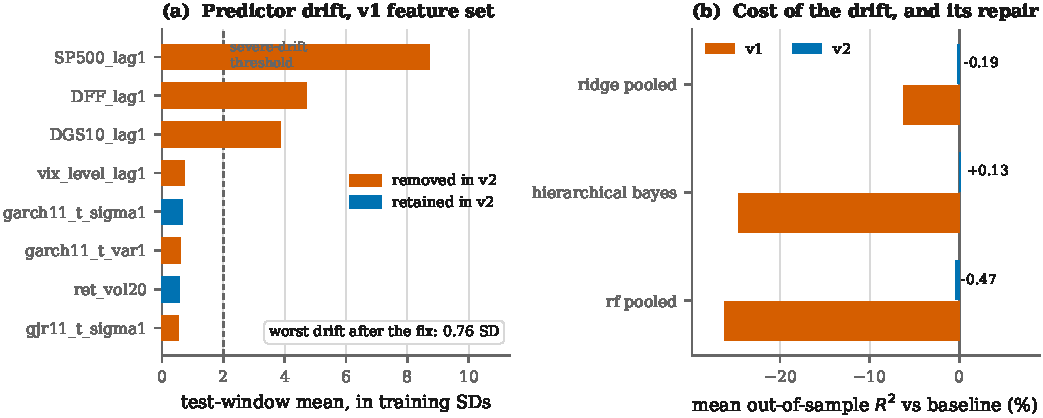
\includegraphics[width=\linewidth]{fig1_extrapolation.pdf}
\caption{Predictor drift and its repair. Panel (a) shows where the test window
sits relative to training moments for the v1 feature set, in training standard
deviations, coloured by whether the corrected specification retains the feature.
Panel (b) shows the mean out-of-sample $R^2$ across the eight tickers before and
after the correction.}
\label{fig:extrapolation}
\end{figure}

\begin{figure}[htbp]
\centering
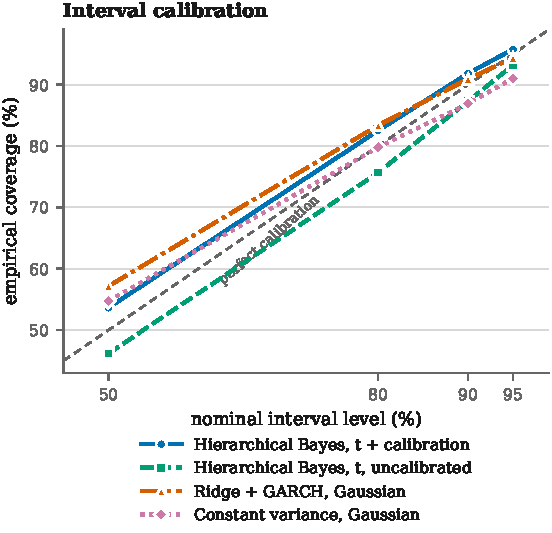
\includegraphics[width=0.62\linewidth]{fig2_reliability.pdf}
\caption{Interval calibration: empirical coverage against nominal level for four
predictive specifications, test window, $n=6008$.}
\label{fig:reliability}
\end{figure}

\begin{figure}[htbp]
\centering
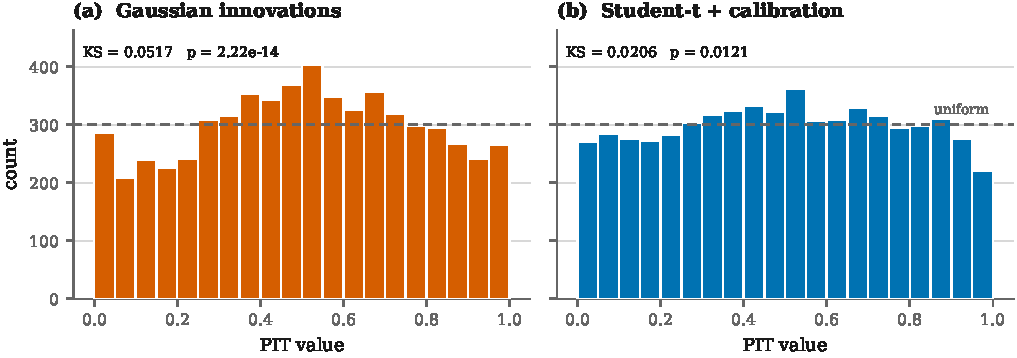
\includegraphics[width=\linewidth]{fig3_pit.pdf}
\caption{Probability integral transform histograms. Under a correctly specified
predictive distribution these are uniform; the dashed line marks the uniform
density and each panel reports a Kolmogorov--Smirnov test against it.}
\label{fig:pit}
\end{figure}

\begin{figure}[htbp]
\centering
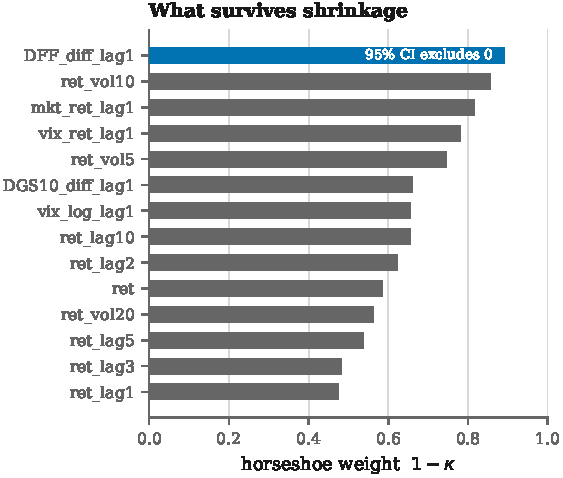
\includegraphics[width=0.75\linewidth]{fig4_shrinkage.pdf}
\caption{Horseshoe shrinkage weight $1-\kappa$ by predictor. Values near one
indicate that the data overrode the prior. The single highlighted predictor has
a $95\%$ credible interval excluding zero.}
\label{fig:shrinkage}
\end{figure}

\begin{figure}[htbp]
\centering
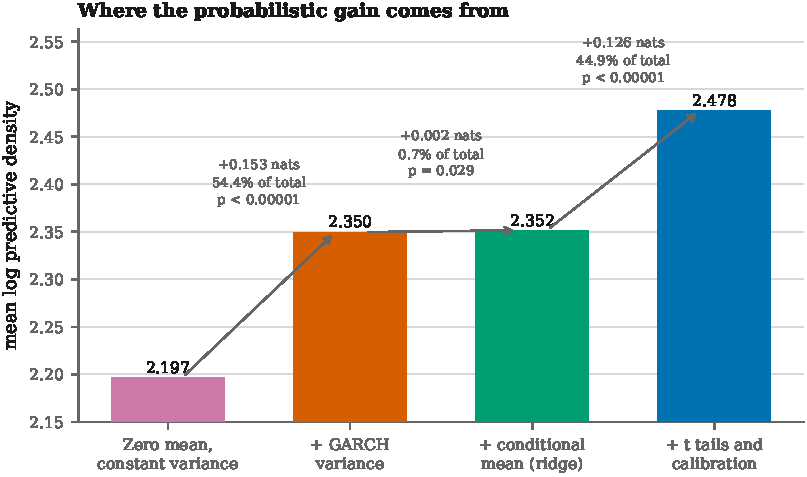
\includegraphics[width=0.8\linewidth]{fig5_decomposition.pdf}
\caption{Decomposition of the gain in mean log predictive density over a null
forecast. Each increment is labelled with its size in nats, its share of the
total gain, and the Diebold--Mariano $p$-value against the preceding rung.}
\label{fig:decomposition}
\end{figure}

% ------------------------------------------------------------- back matter
\section*{Data Availability Statement}
Price data are from Yahoo Finance and macro-financial series from the Federal
Reserve Economic Data service, both publicly available. All code, processed
data, audit scripts and pinned dependencies required to reproduce every number,
table and figure in this paper are available at
\url{https://github.com/RichelCode/Final_Stock_Analysis}.

\section*{Conflict of Interest}
The authors declare no conflict of interest.

\section*{Author Contributions}
\textbf{Author 1:} Conceptualization, Data curation, Methodology, Formal
analysis, Writing -- original draft.
\textbf{Author 2:} Data curation, Methodology, Investigation, Writing --
original draft.
\textbf{Author 3:} Supervision, Project administration, Validation, Writing --
review and editing.

\bibliography{references}

\end{document}
